% !TEX root = ../eval.tex

\section{Results}%
\label{sec:results}

\subsection{Static TWFE}%
\label{sub:static_results}

\begin{equation}
    y_{it} = \alpha_i + \lambda_t + \beta D_{it} + \gamma X_{it} + \epsilon_{it}
\end{equation}

Notes:
\begin{itemize}
    \item Assumption: there are no confounding effects (either time-varying,
        individual varying, or individual-time varying), so treatment
        assignment is as good as random.

    \item With controls, we assume that there are no confounding variables
        other than the ones we control for.
\end{itemize}

\begin{table}[htbp]
   \centering
   \tiny
   \begin{threeparttable}[b]
      \caption{\label{tab:reg_static} Static results}
      \begin{tabular}{lcccccccc}
         \tabularnewline \midrule \midrule
         Dependent Variables: & \multicolumn{4}{c}{Net-inflows} & \multicolumn{4}{c}{Discretionary spend}\\
         Model:          & (1)             & (2)             & (3)            & (4)             & (5)              & (6)             & (7)            & (8)\\  
         \midrule
         \emph{Variables}\\
         App use         & 49.96$^{***}$   & 14.21           & 36.60$^{**}$   & 0.22            & 71.37$^{***}$    & 0.84            & 53.08$^{***}$  & -22.61$^{***}$\\   
                         & [19.11; 80.82]  & [-31.50; 59.92] & [6.08; 67.12]  & [-49.16; 49.61] & [65.39; 77.36]   & [-13.45; 15.13] & [43.96; 62.19] & [-33.62; -11.61]\\   
         Month income    & 0.07$^{***}$    & 0.07$^{***}$    & 0.08$^{***}$   & 0.08$^{***}$    & 0.02$^{***}$     & 0.02$^{***}$    & 0.01$^{***}$   & 0.01$^{***}$\\   
                         & [0.06; 0.08]    & [0.05; 0.09]    & [0.05; 0.10]   & [0.05; 0.11]    & [0.02; 0.02]     & [0.02; 0.03]    & [0.00; 0.02]   & [0.00; 0.01]\\   
         Month spend     & -0.12$^{***}$   & -0.12$^{***}$   & -0.16$^{***}$  & -0.16$^{***}$   & 0.16$^{***}$     & 0.16$^{***}$    & 0.12$^{***}$   & 0.12$^{***}$\\   
                         & [-0.13; -0.11]  & [-0.14; -0.10]  & [-0.18; -0.14] & [-0.19; -0.13]  & [0.16; 0.16]     & [0.15; 0.17]    & [0.11; 0.12]   & [0.11; 0.12]\\   
         Active accounts & 38.80$^{***}$   & 37.49$^{***}$   & 70.26$^{***}$  & 68.78$^{***}$   & 46.84$^{***}$    & 42.56$^{***}$   & 86.86$^{***}$  & 75.18$^{***}$\\   
                         & [30.04; 47.56]  & [23.46; 51.53]  & [53.08; 87.44] & [46.71; 90.85]  & [45.14; 48.54]   & [39.57; 45.55]  & [81.78; 91.95] & [70.63; 79.72]\\   
         Intercept       & -6.05           &                 &                &                 & 171.35$^{***}$   &                 &                &   \\   
                         & [-41.06; 28.95] &                 &                &                 & [164.56; 178.14] &                 &                &   \\   
         \midrule
         \emph{Fixed-effects}\\
         Year-month      &                 & Yes             &                & Yes             &                  & Yes             &                & Yes\\  
         User ID         &                 &                 & Yes            & Yes             &                  &                 & Yes            & Yes\\  
         \midrule
         \emph{Fit statistics}\\
         Observations    & 148,932         & 148,932         & 148,932        & 148,932         & 148,932          & 148,932         & 148,932        & 148,932\\  
         R$^2$           & 0.00879         & 0.00932         & 0.03981        & 0.04033         & 0.41708          & 0.42534         & 0.66066        & 0.66973\\  
         Within R$^2$    &                 & 0.00869         & 0.00933        & 0.00922         &                  & 0.41021         & 0.28163        & 0.23660\\  
         \midrule \midrule
         \multicolumn{9}{l}{\emph{Signif. Codes: ***: 0.01, **: 0.05, *: 0.1}}\\
      \end{tabular}
   \end{threeparttable}
\end{table}





\subsection{Dynamic TWFE}%
\label{sub:dynamic_results}

\begin{equation}
    y_{it} = \alpha_i + \lambda_t + \sum^{5}_{\substack{s=-6 \\
    s\neq-1}} \beta_s D_{its} + \gamma X_{it} + \epsilon_{it},
\end{equation}

where $y_{it}$ is the outcome for individual $i$ at time $t$, $\alpha_i$ and
$\lambda_t$ are individual and year-month fixed effects, respectively, and
$X_{it}$ is a vector of individual and time varying controls. $D_{its}$ equals
1 if, in period $t$, individual $i$ is $s$ months away from signing up to the
app. The set of $\beta_s$ coefficients measure the effect of treatment $s$
periods away from treatment, which is what we are interested in.

We omit the relative period indicator for period $s = -1$ because we need to
omit one relative period indicator to avoid perfect collinearity among the
period indicators, and we choose the last pre-treatment period because it
serves as a natural benchmark against which to compare the outcomes in other
periods.\footnote{As \citet{sun2021estimating} point out, there are two sources
of perfect multicollinearity when estimating a fully dynamic model (i.e. one
including all possible lags). The first results from all relative period
indicators summing to 1 in each period, so that the entire set of relative period
dummies across all time periods is perfectly multicollinear. We deal with this
by excluding the indicator for $s = -1$. The second issue arises from the fact
that for initial treatment period $E_i$, $t = s + E_i$. We deal with this issue
by "trimming" our sample to be balanced in relative periods by only using
data from relative periodl $\{-6, 5\}$. Both of these approaches are standard
in the empirical literature.}


\citet{sun2021estimating} define an event study design as a staggered adoption
design where units are treated at different times and where there may or may
not be never treated units. In our case, we have no never treated units, and
treatment is absorbing in that once a unit is treated they will also be treated
in all subsequent units.\footnote{We cannot rule out that some users who
stopped using the app and closed their account rejoined later on, in which case
they would appear in our dataset as a new user. However, we can plausibly
assume that such cases are rare.} 

Setup:
\begin{itemize}
    \item We observe $N+1$ unites for $T+1$ periods and, for each
        $i\in\{0,\ldots, N\}$ and $t\in\{0,\ldots,T\}$ observe outcome $y_{it}$
        and treatment status $D_{it}\in\{0, 1\}$, where $D_{it}$ equals 1 if unit
        $i$ is treated in period $t$ and 0 otherwise.

    \item We can uniquely characterise treatment paths by the time period of
        initial treatment, denoted as $E_i = min\{t: D_{it} = 1\}$.

    \item We can group units into cohorts $e \in \{0,\ldots, T\}$, where units
        in cohort $e$ were all first treated at time $e$, so that $\{i: E_i =
        e\}$.

    \item We define $y^e_{it}$ as the potential outcome in period $t$ if unit
        $i$ was first treated in period $e$.

\end{itemize}


Assumptions:
\begin{itemize}
    \item Observations $\{y_{it}, D_{it}\}_{t=0}^T$ are independent.

    \item A1: parallel trends: difference in baseline outcomes over time do
        not differ between treatment cohorts. Not obviously violated in our
        context. Early adopters might differ from late adopters, but difference
        might plausibly be constant over time. - We don't have never treated
        units, so Ashenfelter dip scenario is not a problem, even though we
        seem to observe something like this in discretionary spending graph
        (increase in disc spend before signup)

    \item A2: no anticipatory behaviour. Plausibly violated if people are
        motivated to save more and start doing so even before app use. Can test
        for whether there is a peak prior to signup. Because our units have
        private knowledge about future of treatment path (their intention to
        reduce spending and save more and sign up to an app), this might be
        violated. The trajectories of discret spend and net inflows are
        conflicting on this, though, suggesting that they increases discret
        spend in runup to app use (which might provide motivation to eventually
        sign up) but also might have increased net savings slightly.

    \item A3: treatment effect homogeneity across all cohorts and all relative
        periods. (Note: treatment effects can be dynamic, but need to be the
        same across cohorts). We could test for this.

\end{itemize}


Notes:
\begin{itemize}

    \item Comparison: pre vs post signup within each individual.

    \item Assumption: there are no time-varying unobserved effects that affect
        both y and D (formally: $E[Du] = 0$, since u is by definition
        correlated with y.

    \item Discussion: there is something that made the individual sign up in
        the first place, and it might well be an individual level shock that we
        don't observe (unexpected large expense, loss of job, exposure to
        something that motivates saving or change in financial behaviour).

    \item See \citet{imai2021use} for problems with twfe

\end{itemize}


\begin{table}[htbp]
   \centering
   \tiny
   \begin{threeparttable}[b]
      \caption{\label{tab:reg_dynamic} Dynamic results}
      \begin{tabular}{lcccccccc}
         \tabularnewline \midrule \midrule
         Dependent Variables: & \multicolumn{4}{c}{Net-inflows} & \multicolumn{4}{c}{Discretionary spend}\\
         Model:                          & (1)               & (2)               & (3)               & (4)               & (5)                & (6)              & (7)                & (8)\\  
         \midrule
         \emph{Variables}\\
         Months to/since app use $=$ <-6 & -110.84$^{***}$   & -103.66$^{*}$     & -98.69$^{**}$     & -89.62$^{*}$      & -125.40$^{***}$    & -78.16$^{***}$   & -118.87$^{***}$    & -59.75$^{***}$\\   
                                         & [-194.27; -27.42] & [-208.63; 1.30]   & [-196.09; -1.30]  & [-195.15; 15.91]  & [-141.55; -109.25] & [-90.83; -65.49] & [-133.11; -104.63] & [-75.32; -44.18]\\   
         Months to/since app use $=$ -5  & -35.38            & -33.48            & -32.47            & -29.27            & -75.75$^{***}$     & -54.58$^{***}$   & -70.92$^{***}$     & -45.70$^{***}$\\   
                                         & [-147.30; 76.55]  & [-104.30; 37.33]  & [-157.19; 92.26]  & [-101.94; 43.41]  & [-97.42; -54.08]   & [-75.39; -33.77] & [-86.97; -54.88]   & [-60.92; -30.48]\\   
         Months to/since app use $=$ -4  & -84.56            & -72.77            & -83.59            & -70.73            & -57.64$^{***}$     & -35.26$^{***}$   & -55.23$^{***}$     & -29.49$^{***}$\\   
                                         & [-196.42; 27.31]  & [-210.15; 64.60]  & [-209.56; 42.39]  & [-199.69; 58.23]  & [-79.30; -35.98]   & [-51.02; -19.50] & [-70.63; -39.82]   & [-42.97; -16.00]\\   
         Months to/since app use $=$ -3  & -71.07            & -62.18            & -70.38            & -60.24            & -30.29$^{***}$     & -14.47           & -28.66$^{***}$     & -9.71\\   
                                         & [-182.90; 40.75]  & [-170.79; 46.43]  & [-199.96; 59.20]  & [-173.35; 52.87]  & [-51.94; -8.63]    & [-32.82; 3.87]   & [-43.89; -13.44]   & [-28.77; 9.36]\\   
         Months to/since app use $=$ -2  & -122.75$^{**}$    & -119.55$^{**}$    & -122.03$^{**}$    & -118.23$^{**}$    & -4.43              & -1.01            & -2.94              & 1.77\\   
                                         & [-234.56; -10.93] & [-225.23; -13.87] & [-243.52; -0.54]  & [-216.49; -19.96] & [-26.08; 17.22]    & [-18.48; 16.47]  & [-17.65; 11.78]    & [-13.53; 17.06]\\   
         Months to/since app use $=$ 0   & -21.42            & -11.68            & -26.70            & -15.70            & -45.13$^{***}$     & -31.21$^{***}$   & -51.60$^{***}$     & -36.62$^{***}$\\   
                                         & [-133.23; 90.40]  & [-111.40; 88.05]  & [-154.64; 101.24] & [-113.59; 82.19]  & [-66.78; -23.48]   & [-47.29; -15.14] & [-66.74; -36.47]   & [-51.09; -22.15]\\   
         Months to/since app use $=$ 1   & -58.47            & -62.50            & -62.12            & -63.71            & -40.35$^{***}$     & -34.83$^{***}$   & -44.46$^{***}$     & -38.80$^{***}$\\   
                                         & [-170.30; 53.36]  & [-182.33; 57.34]  & [-189.27; 65.03]  & [-176.44; 49.01]  & [-62.01; -18.70]   & [-53.64; -16.02] & [-60.03; -28.88]   & [-57.74; -19.87]\\   
         Months to/since app use $=$ 2   & -122.16$^{**}$    & -128.48$^{**}$    & -124.56$^{**}$    & -128.78$^{**}$    & -27.21$^{**}$      & -34.63$^{**}$    & -30.15$^{***}$     & -39.25$^{***}$\\   
                                         & [-234.00; -10.31] & [-241.72; -15.24] & [-245.46; -3.66]  & [-240.72; -16.84] & [-48.87; -5.56]    & [-61.44; -7.83]  & [-46.11; -14.18]   & [-62.98; -15.53]\\   
         Months to/since app use $=$ 3   & -55.31            & -66.69            & -57.53            & -66.80            & -27.30$^{**}$      & -43.86$^{***}$   & -30.16$^{***}$     & -49.35$^{***}$\\   
                                         & [-167.18; 56.55]  & [-184.08; 50.71]  & [-176.91; 61.85]  & [-174.31; 40.72]  & [-48.96; -5.64]    & [-64.72; -22.99] & [-46.04; -14.28]   & [-66.78; -31.91]\\   
         Months to/since app use $=$ 4   & -85.94            & -97.30            & -87.90            & -96.92            & -23.89$^{**}$      & -37.71$^{***}$   & -26.92$^{***}$     & -43.08$^{***}$\\   
                                         & [-197.82; 25.94]  & [-219.28; 24.68]  & [-207.50; 31.69]  & [-219.67; 25.83]  & [-45.55; -2.22]    & [-60.17; -15.24] & [-42.85; -10.00]   & [-58.87; -27.29]\\   
         Months to/since app use $=$ 5   & 46.03             & 33.02             & 44.40             & 34.50             & -25.47$^{**}$      & -36.66$^{***}$   & -28.84$^{***}$     & -41.60$^{***}$\\   
                                         & [-65.87; 157.93]  & [-100.42; 166.46] & [-76.21; 165.01]  & [-95.93; 164.93]  & [-47.13; -3.80]    & [-56.31; -17.02] & [-45.14; -12.53]   & [-59.75; -23.46]\\   
         Months to/since app use $=$ >5  & -39.39            & -63.30            & -40.34            & -62.71            & -13.55             & -41.94$^{***}$   & -22.44$^{***}$     & -61.44$^{***}$\\   
                                         & [-125.16; 46.38]  & [-171.70; 45.11]  & [-138.79; 58.11]  & [-176.22; 50.79]  & [-30.16; 3.05]     & [-59.32; -24.57] & [-37.23; -7.65]    & [-80.30; -42.58]\\   
         Month income                    & 0.07$^{***}$      & 0.07$^{***}$      & 0.08$^{***}$      & 0.08$^{***}$      & 0.02$^{***}$       & 0.02$^{***}$     & 0.01$^{***}$       & 0.01$^{***}$\\   
                                         & [0.06; 0.08]      & [0.05; 0.09]      & [0.05; 0.10]      & [0.05; 0.11]      & [0.02; 0.02]       & [0.02; 0.03]     & [0.01; 0.02]       & [0.00; 0.01]\\   
         Month spend                     & -0.12$^{***}$     & -0.12$^{***}$     & -0.16$^{***}$     & -0.16$^{***}$     & 0.16$^{***}$       & 0.16$^{***}$     & 0.12$^{***}$       & 0.12$^{***}$\\   
                                         & [-0.13; -0.11]    & [-0.14; -0.10]    & [-0.18; -0.14]    & [-0.19; -0.13]    & [0.16; 0.16]       & [0.15; 0.17]     & [0.11; 0.12]       & [0.11; 0.12]\\   
         Active accounts                 & 36.80$^{***}$     & 36.50$^{***}$     & 67.24$^{***}$     & 67.15$^{***}$     & 42.73$^{***}$      & 41.25$^{***}$    & 78.73$^{***}$      & 72.40$^{***}$\\   
                                         & [27.80; 45.80]    & [22.39; 50.60]    & [49.37; 85.11]    & [45.29; 89.01]    & [40.98; 44.47]     & [38.24; 44.26]   & [73.58; 83.88]     & [67.44; 77.35]\\   
         Intercept                       & 93.70$^{**}$      &                   &                   &                   & 276.72$^{***}$     &                  &                    &   \\   
                                         & [6.98; 180.42]    &                   &                   &                   & [259.93; 293.52]   &                  &                    &   \\   
         \midrule
         \emph{Fixed-effects}\\
         Year-month                      &                   & Yes               &                   & Yes               &                    & Yes              &                    & Yes\\  
         User ID                         &                   &                   & Yes               & Yes               &                    &                  & Yes                & Yes\\  
         \midrule
         \emph{Fit statistics}\\
         Observations                    & 148,932           & 148,932           & 148,932           & 148,932           & 148,932            & 148,932          & 148,932            & 148,932\\  
         R$^2$                           & 0.00892           & 0.00944           & 0.03993           & 0.04044           & 0.41920            & 0.42596          & 0.66235            & 0.67014\\  
         Within R$^2$                    &                   & 0.00881           & 0.00945           & 0.00933           &                    & 0.41085          & 0.28520            & 0.23755\\  
         \midrule \midrule
         \multicolumn{9}{l}{\emph{Signif. Codes: ***: 0.01, **: 0.05, *: 0.1}}\\
      \end{tabular}
   \end{threeparttable}
\end{table}




\begin{figure}[H]
    \centering
    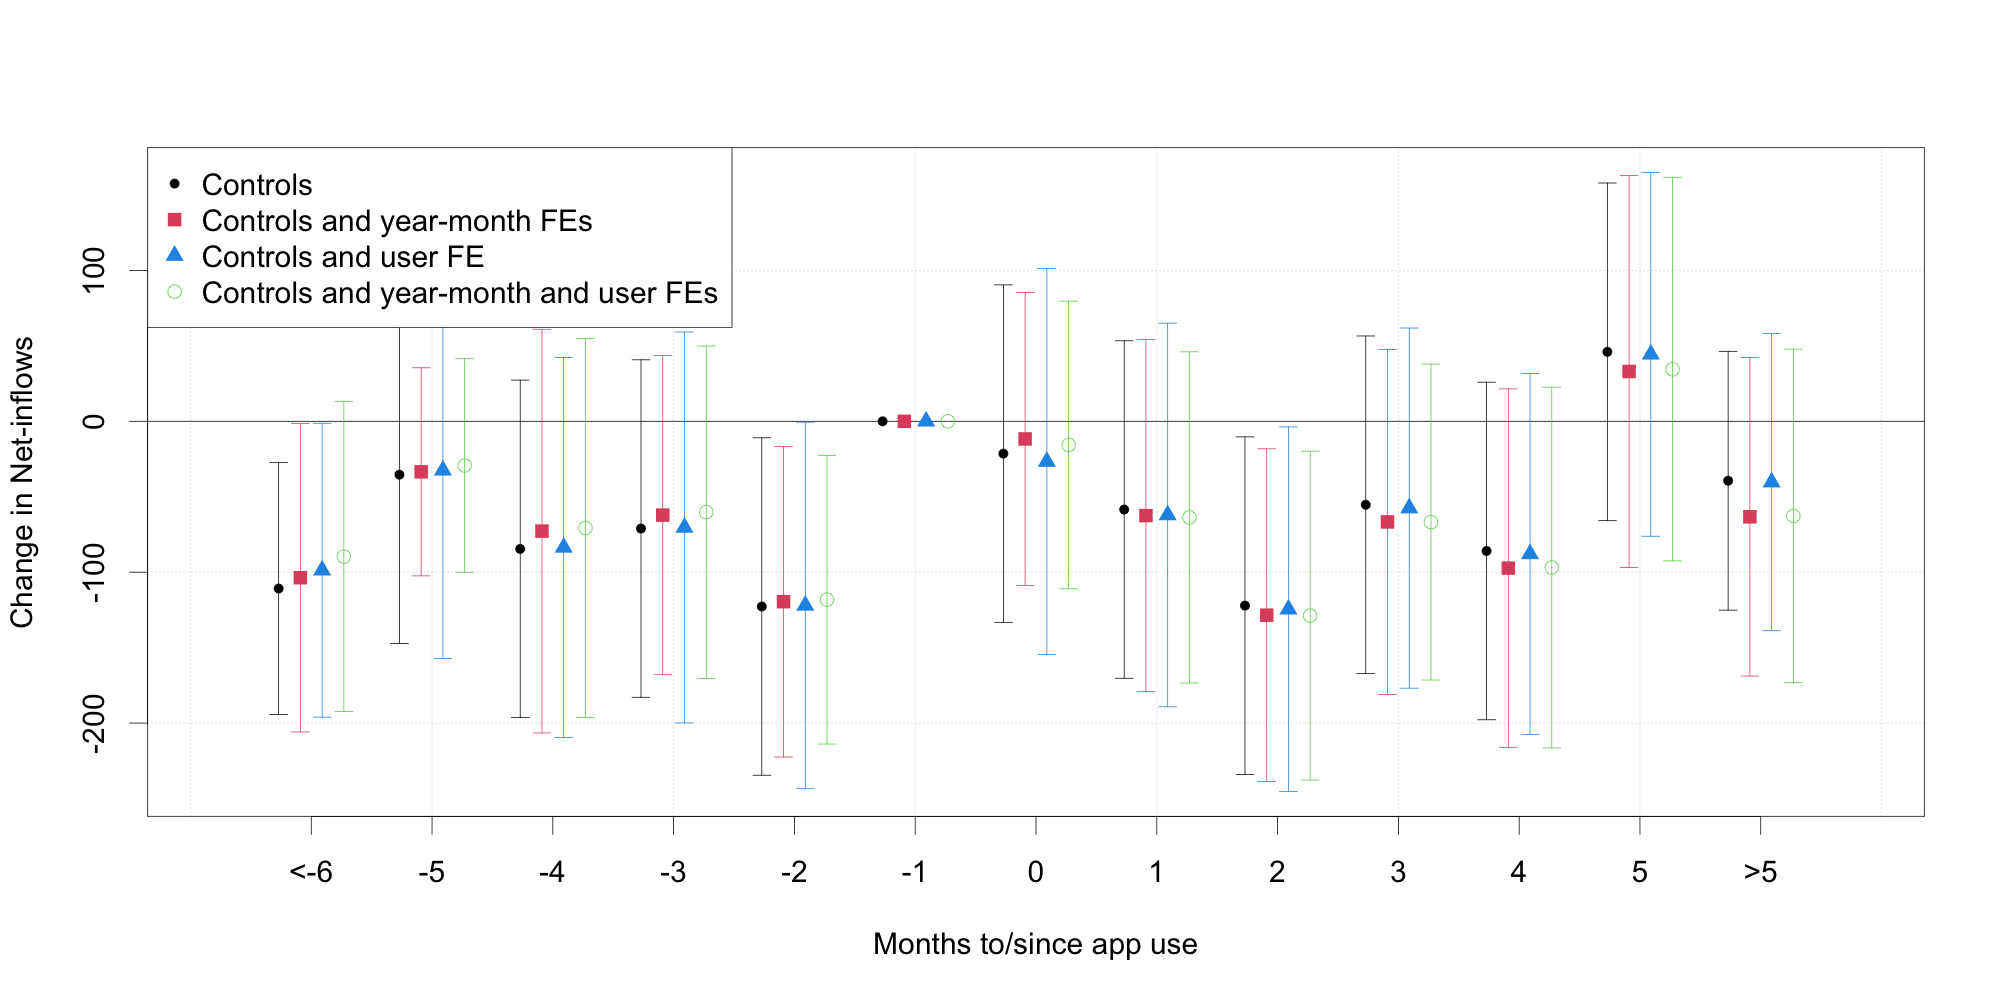
\includegraphics[width=\linewidth]{\figdir/reg_dynamic.png}
    \caption{Dynamic results}%
    \label{fig:reg_dynamic}
\end{figure}


\subsection{Decomposing inflows and outflows}%
\label{sub:decomposing_inflows_and_outflows}

\begin{figure}[H]
    \centering
    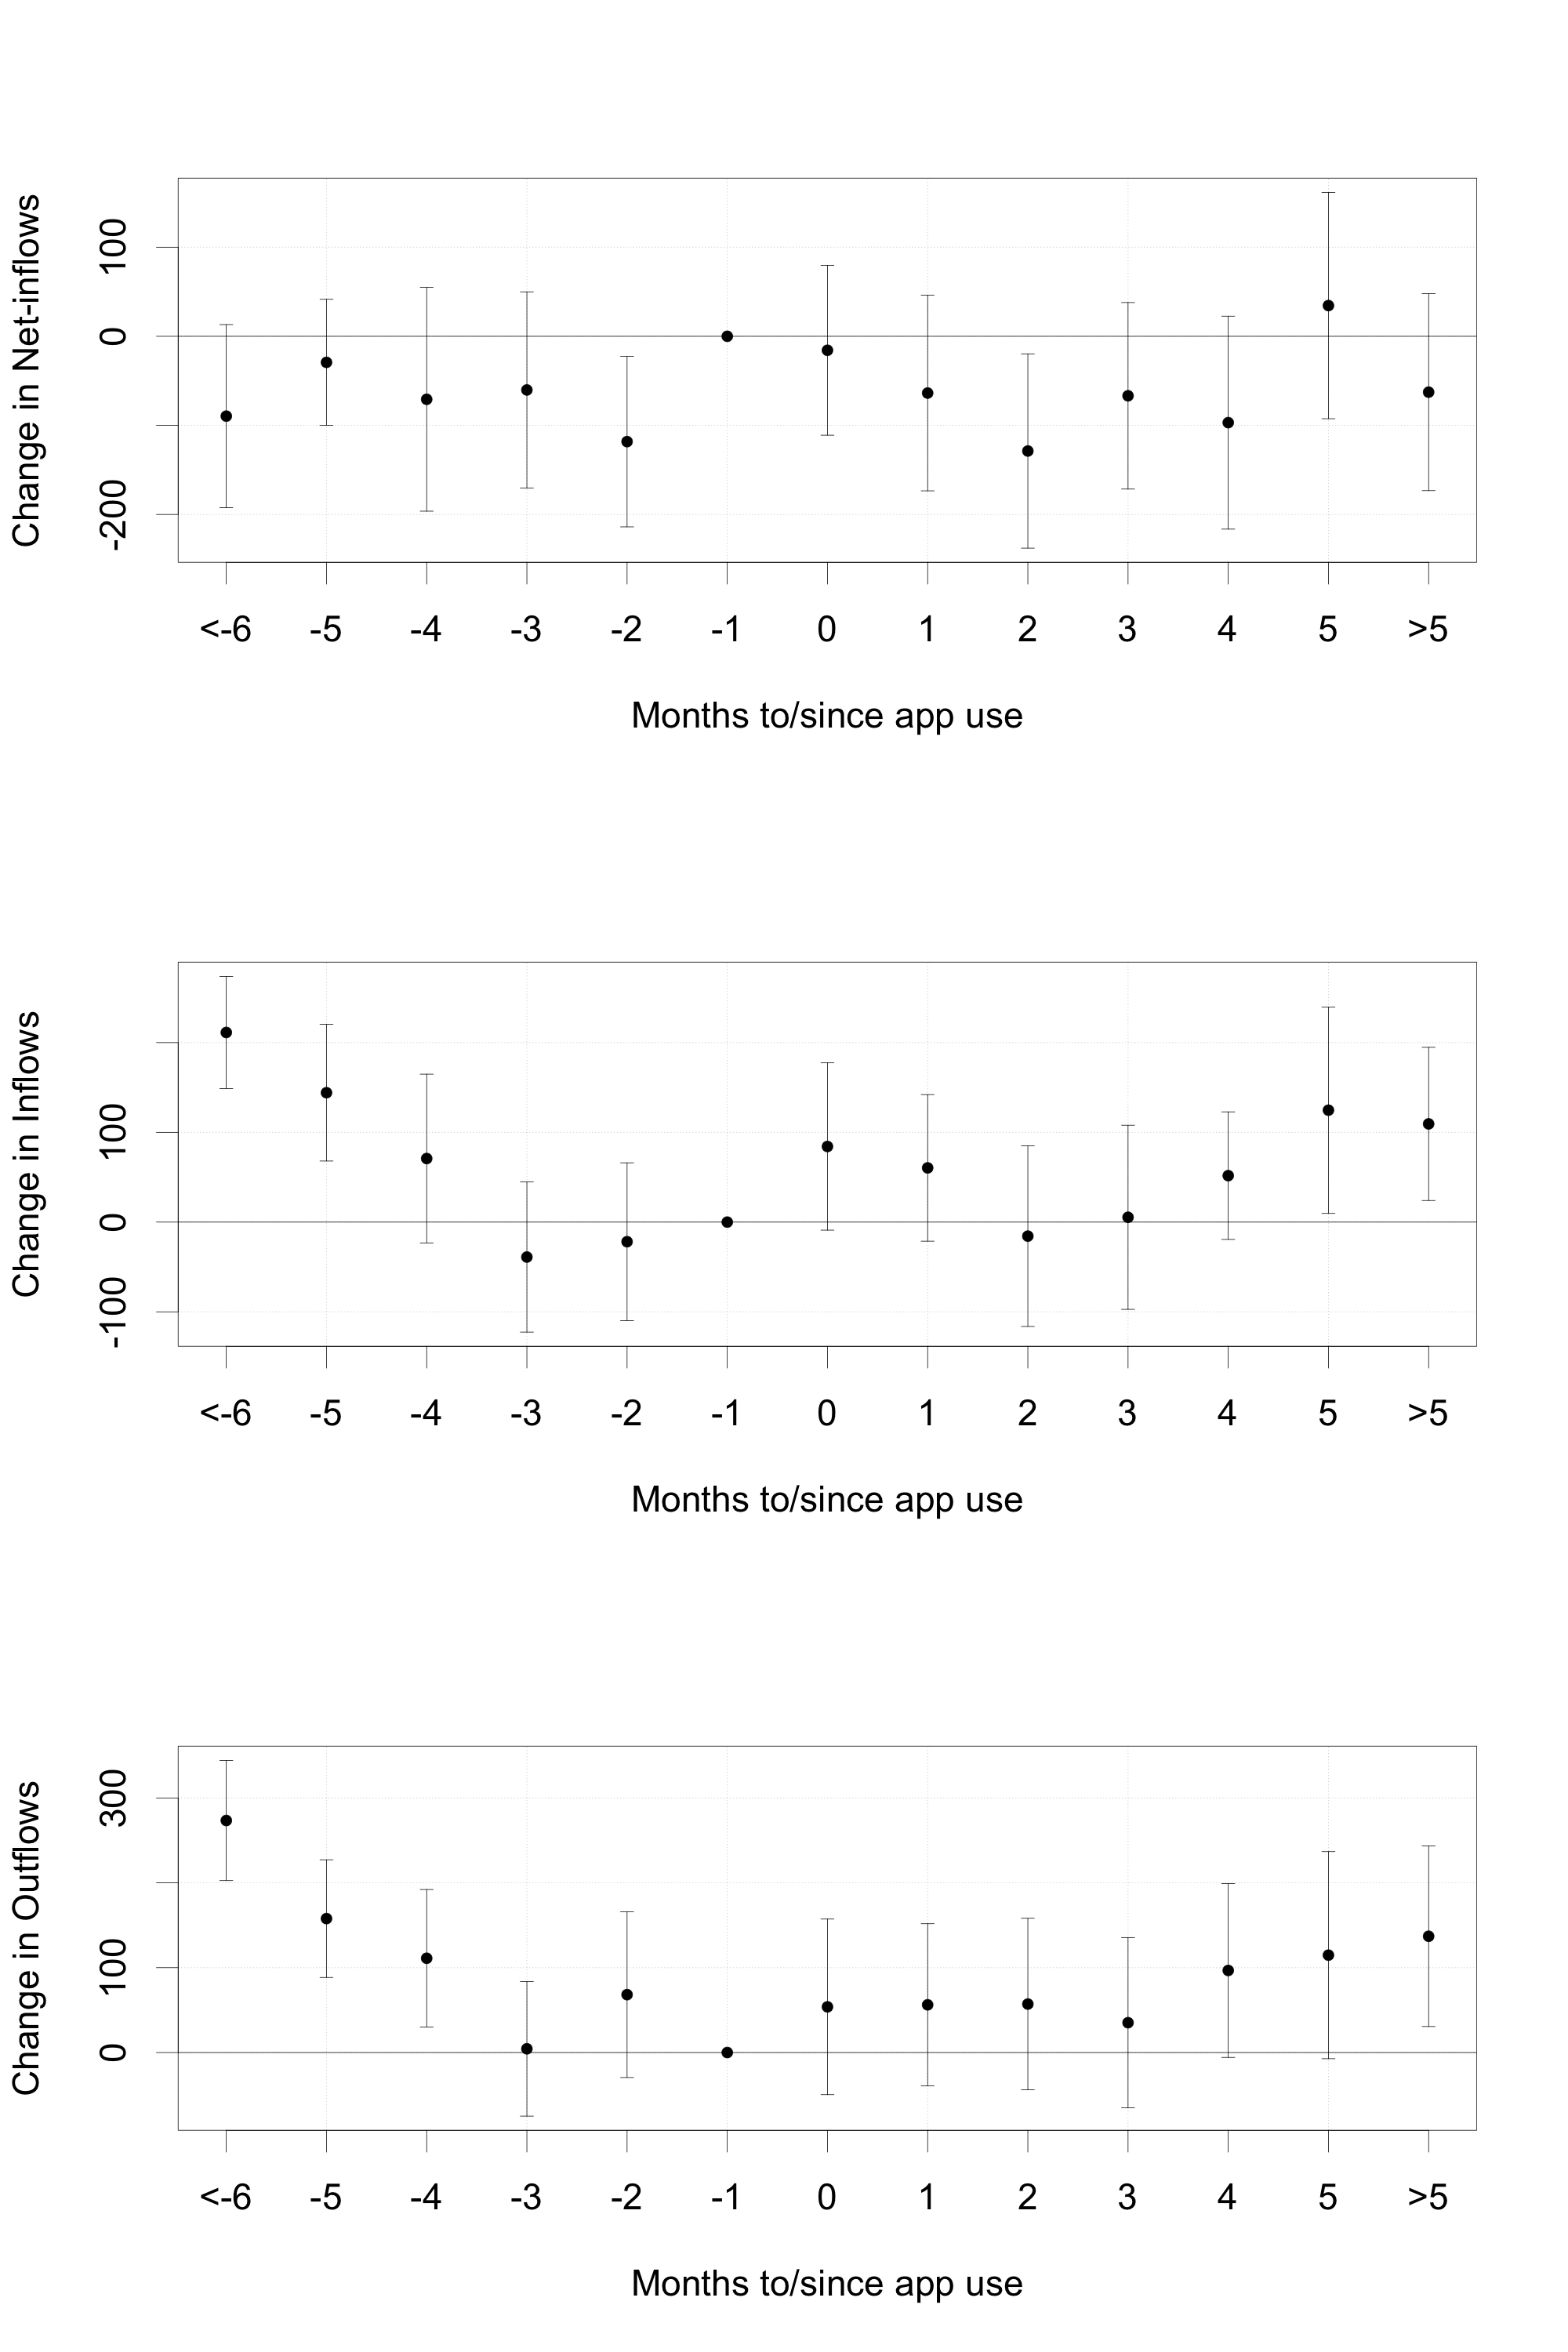
\includegraphics[width=.7\textwidth]{\figdir/reg_decomp_inout}
    \caption{Decomposing inflows and outflows}%
    \label{fig:reg_decomp_inout}
\end{figure}


\subsection{Decomposing intensive and extensive margins}%
\label{sub:decomposing_intensive_and_extensive_margins}

\begin{figure}[H]
    \centering
    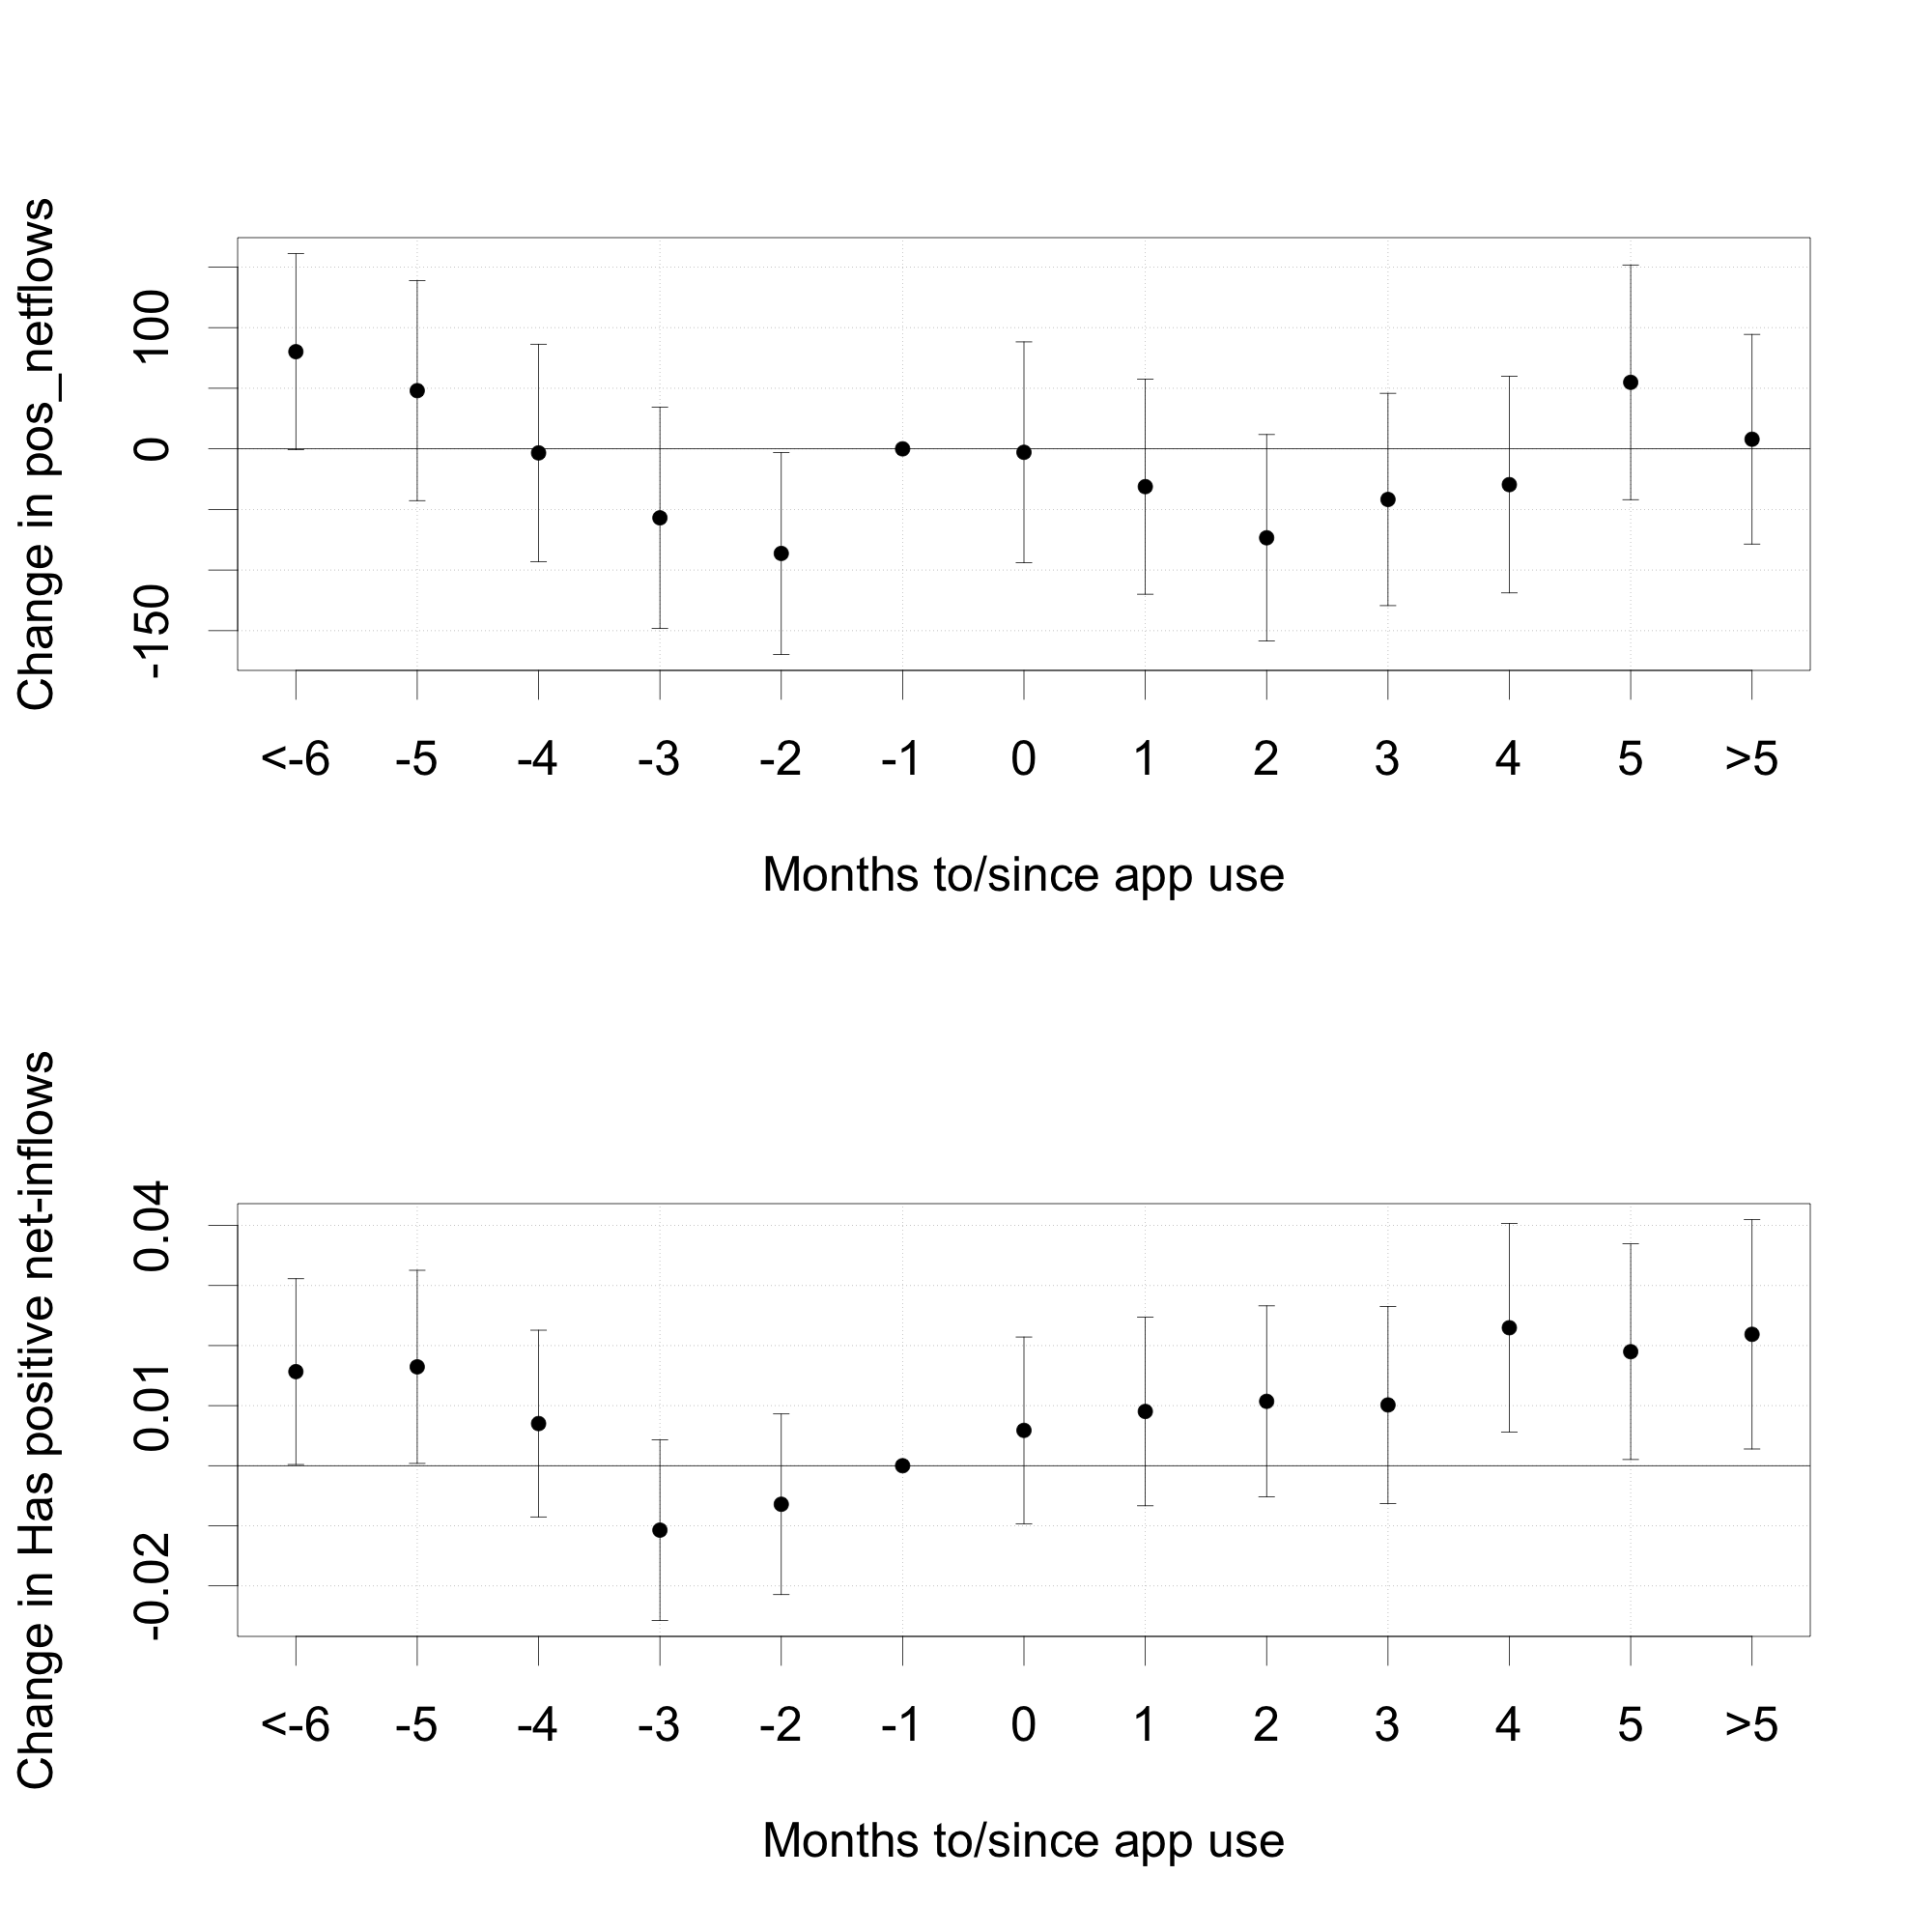
\includegraphics[width=.7\textwidth]{\figdir/reg_decomp_intext}
    \caption{Decomposing intensive and extensive margin}%
    \label{fig:reg_decomp_intext}
\end{figure}


\subsection{Matching}%
\label{sub:alternative_matching_method}

Control group design:
\begin{itemize}

    \item We only have data for a self-selected group of people who choose to
        use the app. This has a couple consequences:

    \item By virtue of signing up to an app that helps them manage
        their money, these users are different from those who don't
        sign up. As a result, we are unable to answer the question of
        whether app use helps the average person in the
        population as a whole save more.\footnote{One way to get closer
            to that answer is to re-weight our sample on observable
            demographic variables so as to match the UK population as a
            whole. But our sample differs from the population as a
            whole both is ways that are observable (demographic
            variables) and unobservable (self-awareness that they need
            help managing their money, cognitive resources to engage
            with the app, motivation to do so). Re-weighting would only
            help us deal with the first of these.}

    \item Even among people who do eventually sign up to the app,
        hte decision when to do so is unlikely to be random --
        \textit{something} makes them sign up at the particular
        point in time they do and not before or after. If we think
        of this factor as ``motivation to save more'', then said
        motivation is inextricably linked with the decision to sign
        up so that we cannot differentiate between the two.

    \item Hence: due to the first point above, we cannot estimate
        an ATE (effect of app use on the average citizen), and due
        to the second point we also cannot estimate a pure ATT
        (effect of app use on users). Instead, our estimated effect
        of app use captures the effect of being motivated to save
        more and using the app to do so.\footnote{One way to get a
            step closer to ATT would be to find a variable that
        correlates with ``motivation to save'' and control for it /
    match on it.}

    \item This is true for both our matched DiD and our TWFE
        design. While these two approaches use a different
        counterfactual to estimate the effect of app use
        (behaviour of a matched control in the case of DiD and
        extrapolating within-user pre-signup behaviour in the case
        of TWFE), neither can help us with the fact that the
        decision to sign up is likely correlated with the
        time-varying unobserved effect ``motivation to save more''.

\end{itemize}

DiD:
\begin{itemize}

    \item We use a difference-in-differences design to estimate the effect of
        app use. Because we do not have a separate control group, we use the
        per-signup data of Money Dashboard users as control periods and use
        matching to find comparable control user for each tretment user.

    \item To do this, we use the matching estimator for panel data proposed by
        \citet{imai2021matching}. Following paper, we conduct the following
        steps:

    \item For each treated observation, we find a set of control observations
        with that share the same treatment history for a period of $L$ periods
        before the treatment and $F$ periods after the treatment. In our
        baseline specification, we rely on a year's worth of data around the
        treatment period and set $L=6$ and $F = 0, 1, 2, 3, 4, 5$.

    \item Identification assumption is that potential outcomes only depend on
        treatment status of the past L periods. In general, this means that if
        treatment has a cumulative effect over time, the full effect is reached
        after L periods. In our context, this means that any effect on savings
        behaviour from usign the app is fully realised after L periods. (I
        think this means that if we look at the treatment effect for F periods
        forward, the effect should not become stronger after F = L).

\end{itemize}

DiD identification assumptions:
\begin{itemize}
    \item No spillover effects: the potential outcome of unit $i$ at time $t$
        is independent of the treatment status of other units. This is violated
        if a user's partner or friends also use the app and, through sharing
        their experiences or motivations, influence the user's savings
        behaviour.

    \item Carryover effects no longer than $L$ periods: a user's potential
        outcome in period $t$ is independent of treatment status in periods
        more than $L$ periods ago. Given that we are dealing with an absorbing
        treatment, this is not a very strong assumption in our context, and we
        choose $L$ based on what we think is an informative number of periods
        to observe pre-app use behaviour.\footnote{An absorbing treatment is
            one that cannot be reversed, and hence we only change from
            untreated to treated once.}.

    \item Parallel trends: the spending trajectory between treated and control
        units would have continued to be parallel if the treated unit hadn't
        started using the app. This is violated whenever an intended change in
        savings behaviour also provided the impetus for the user to start using
        the app, which is likely to occurr frequently. To the extent this is
        the case, we have an ommitted variable ``motivation to save more'',
        which both changes the user's savings behaviour and their treatment
        status. Because of this, what we are measuring is not a pure ATT of app
        use -- the effect of app use on savings over and above the change
        precipitated by a change motivation -- but the effect of app use for
        users motivated to save more.

\end{itemize}


\begin{figure}[H]
    \centering
    \caption{Match set examples}%
    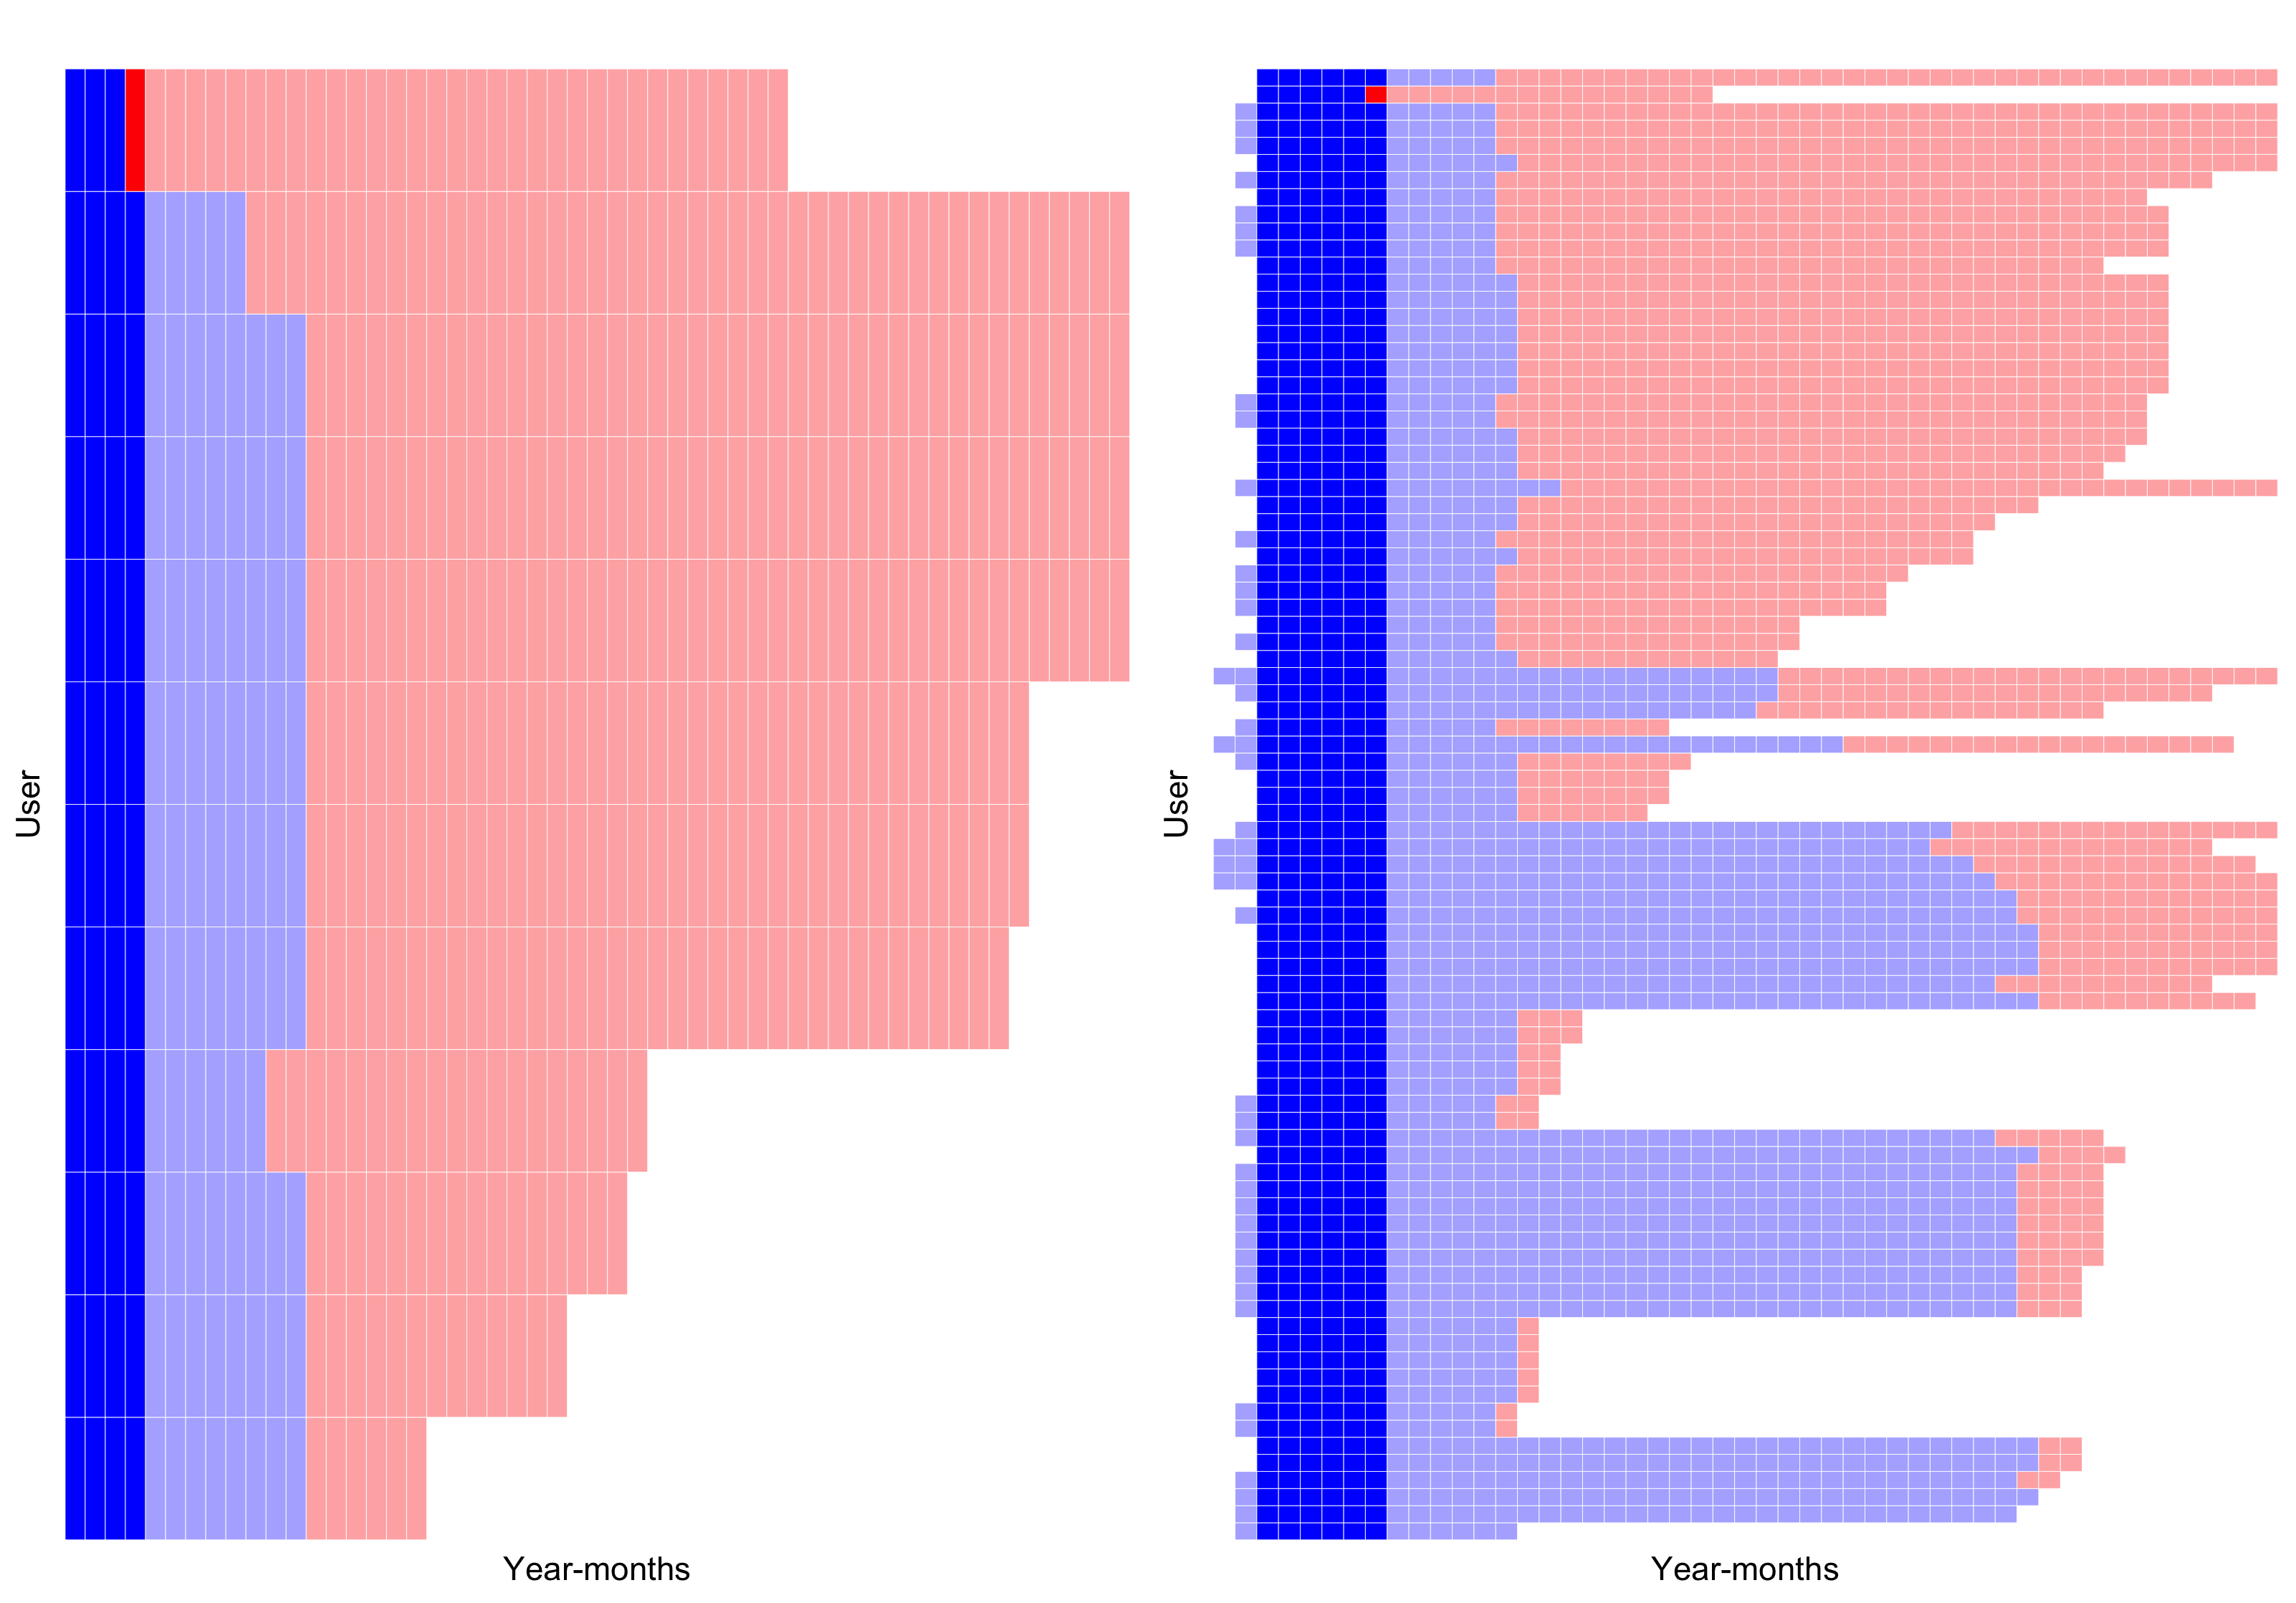
\includegraphics[width=\linewidth]{\figdir/matchset_examples.png}
    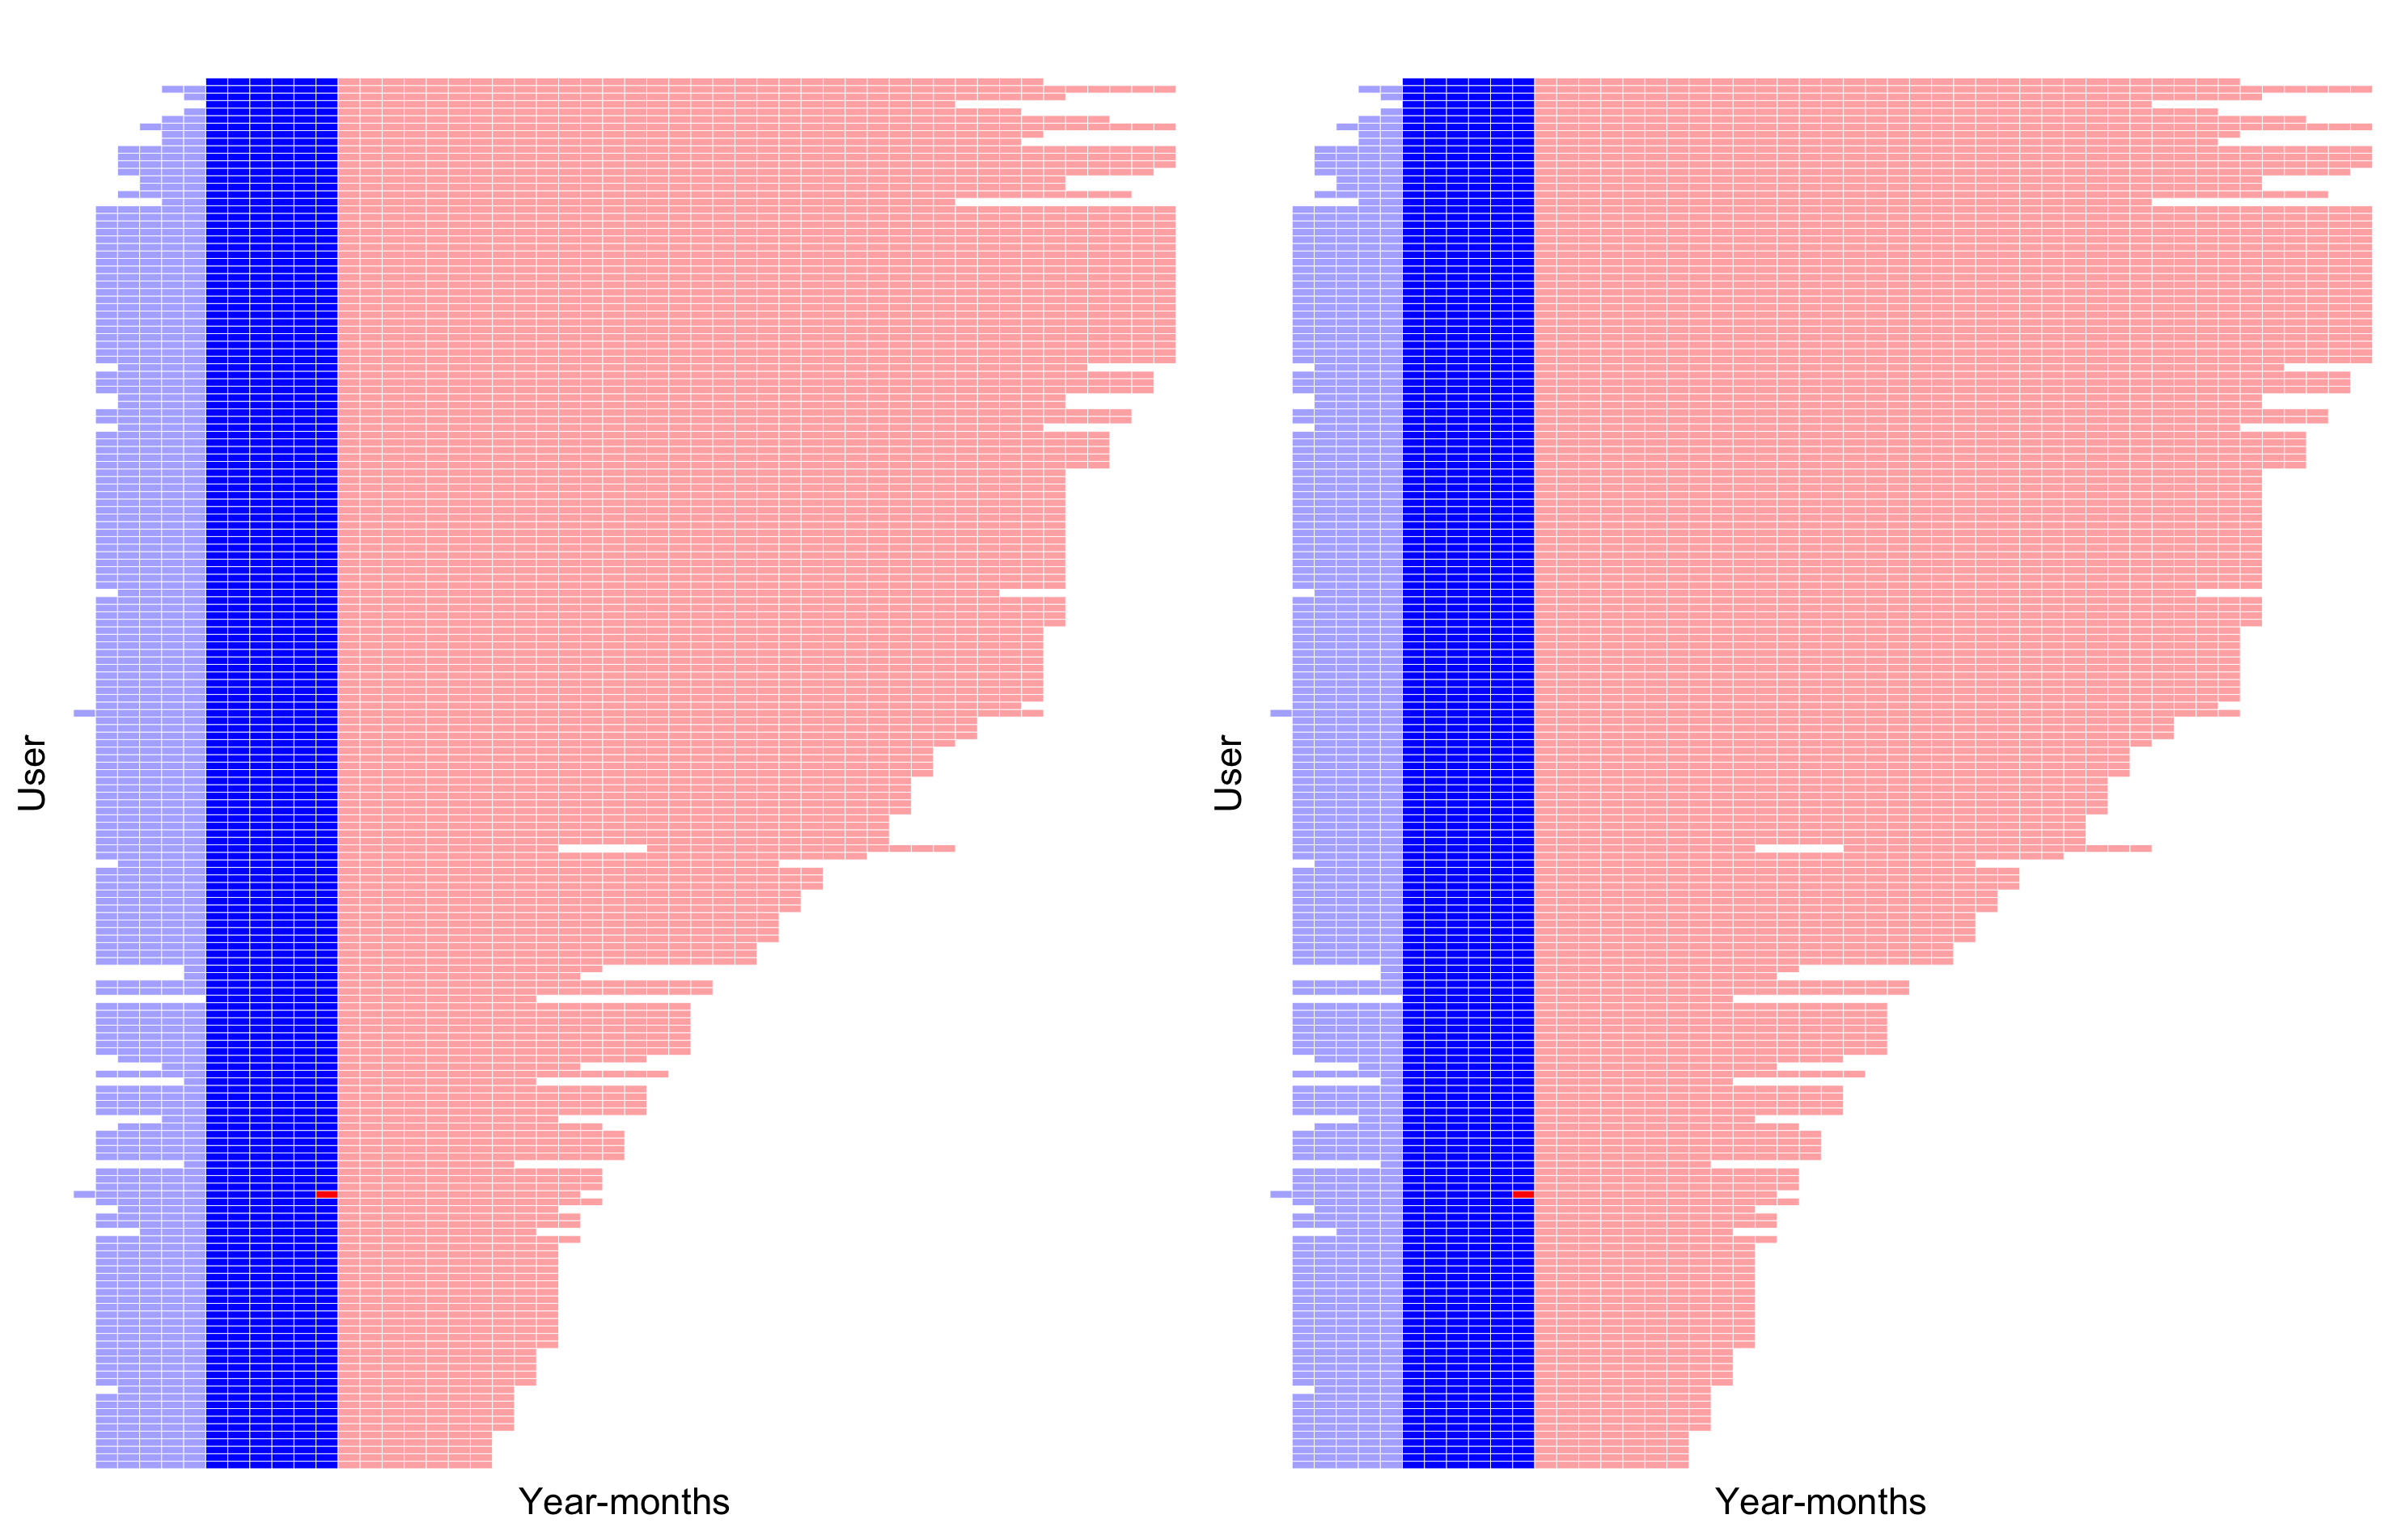
\includegraphics[width=\linewidth]{\figdir/matchset_examples_new.png}
    \label{fig:matchset_examples}

    \fignote{\textwidth}{}

\end{figure}


\begin{figure}[H]
    \centering
    \caption{Distribution of size of matched control units}%
    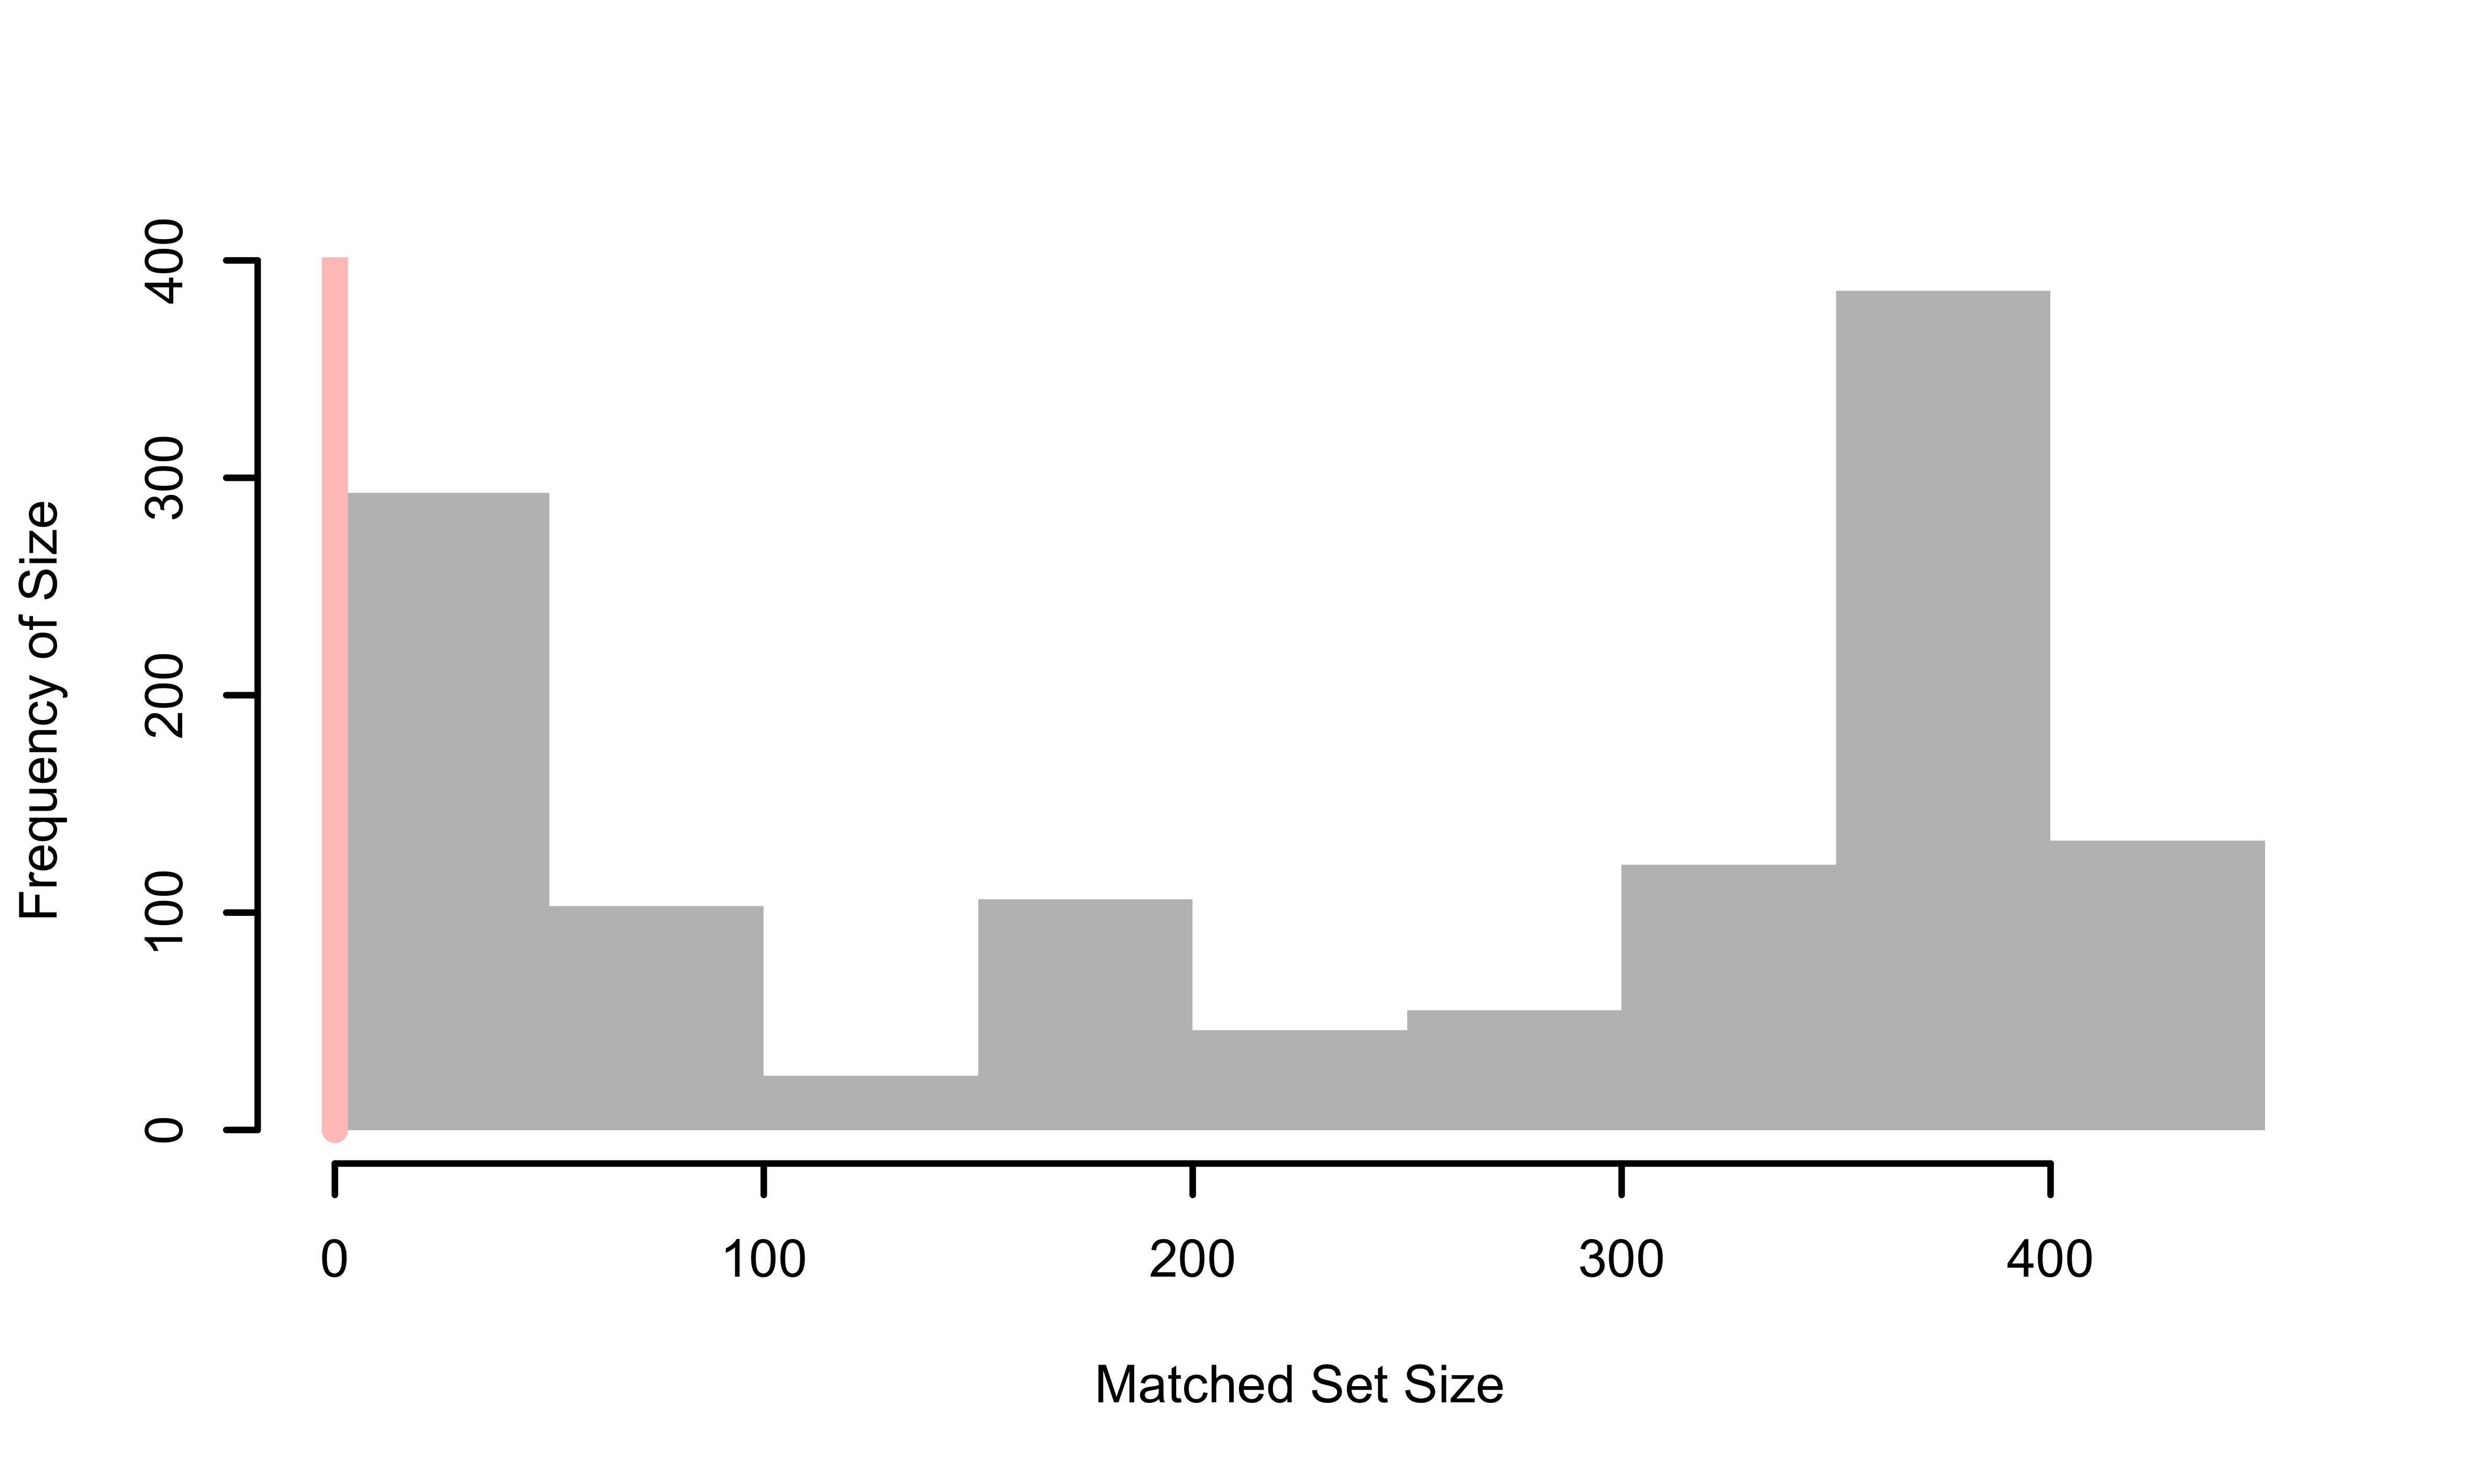
\includegraphics[width=0.8\linewidth]{\figdir/hist_matchset_size.png}
    \label{fig:hist_matchset_size}

    \fignote{\textwidth}{In the first step of the matching proceedure, each
        user gets assigned a set of potential control users that share the same
        treatment history for a specified number of periods before the user
        signs up to teh app (6 months, in our baseline specification), but that
        do not sign up themselves for a specified number of periods after the
        treatment user has signed up (another 6 months, in our baseline
        specification). The figure shows the distribution of the sizes of these
        sets of potential control users. The pink vertical bar on the left
    shows to count of users for whom no control users cound be found.}

\end{figure}

\begin{figure}[H]
    \centering
    \caption{Covariance balance}%
    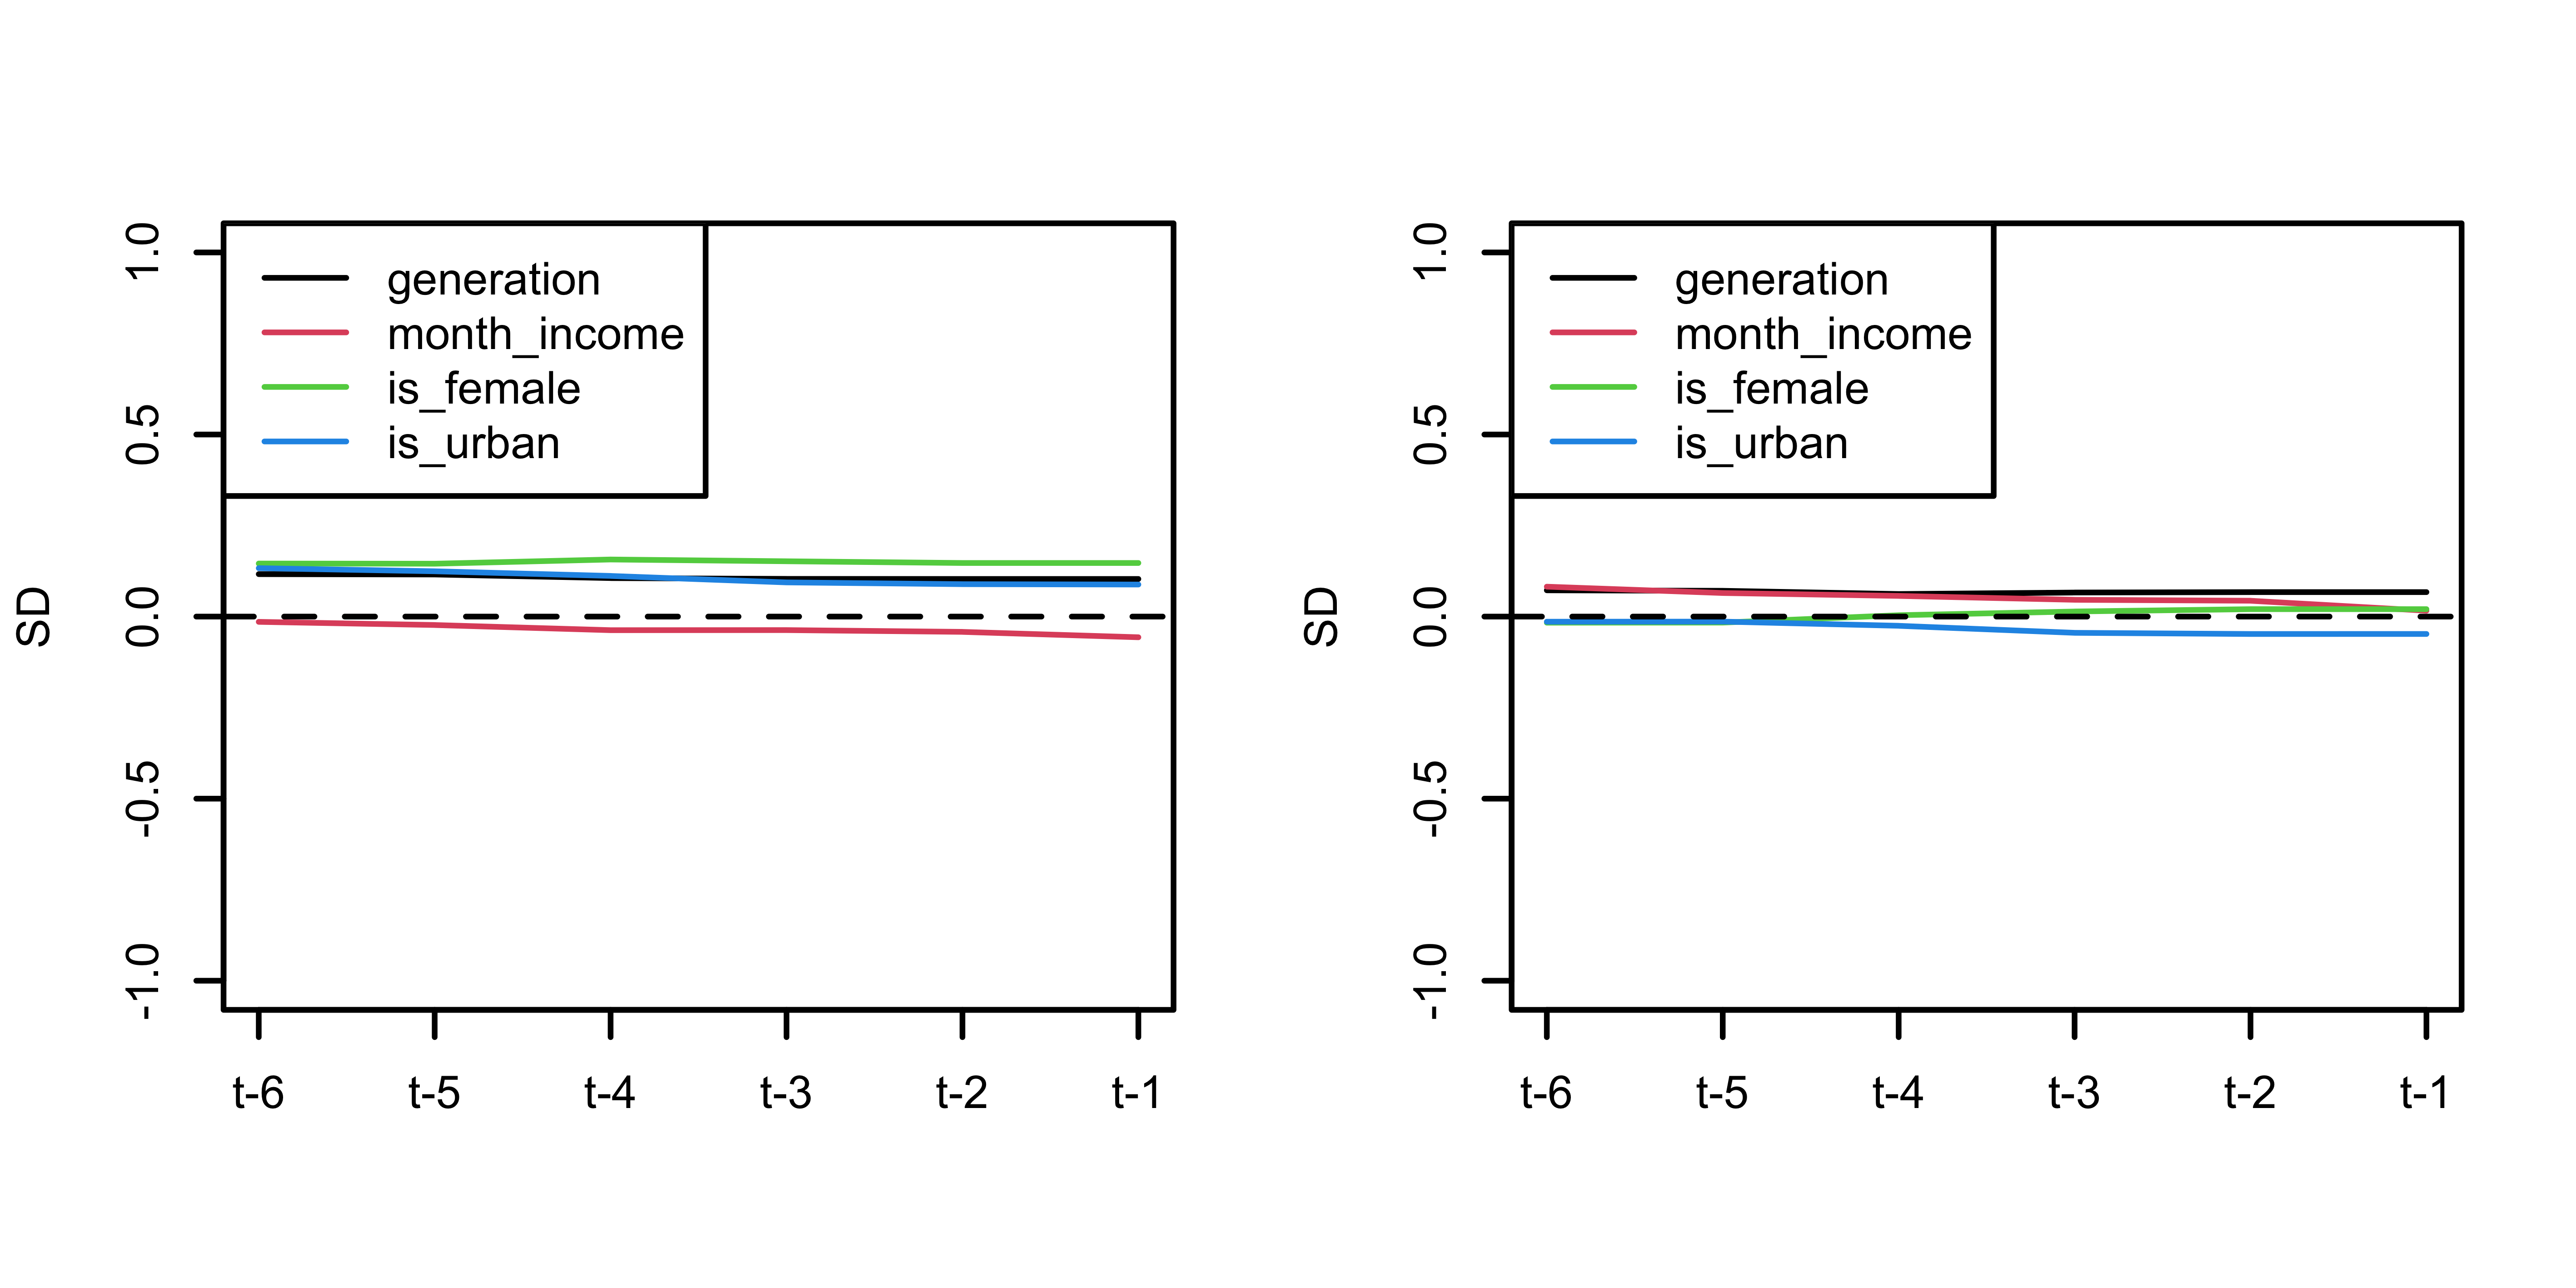
\includegraphics[width=0.8\linewidth]{\figdir/covar_balance.png}
    \label{fig:covar_balance}

    \fignote{\textwidth}{Average covariate standard deviation between treatment and
        control units for each pre-treatment period using the entire set of
        potential controls on the left and, on the right, the refined set of
        controls, which, in our baseline specification, consists of the nearest
        neighbour match based on the propensity score.}

\end{figure}

\begin{figure}[H]
    \centering
    \caption{Matching estimates}%
    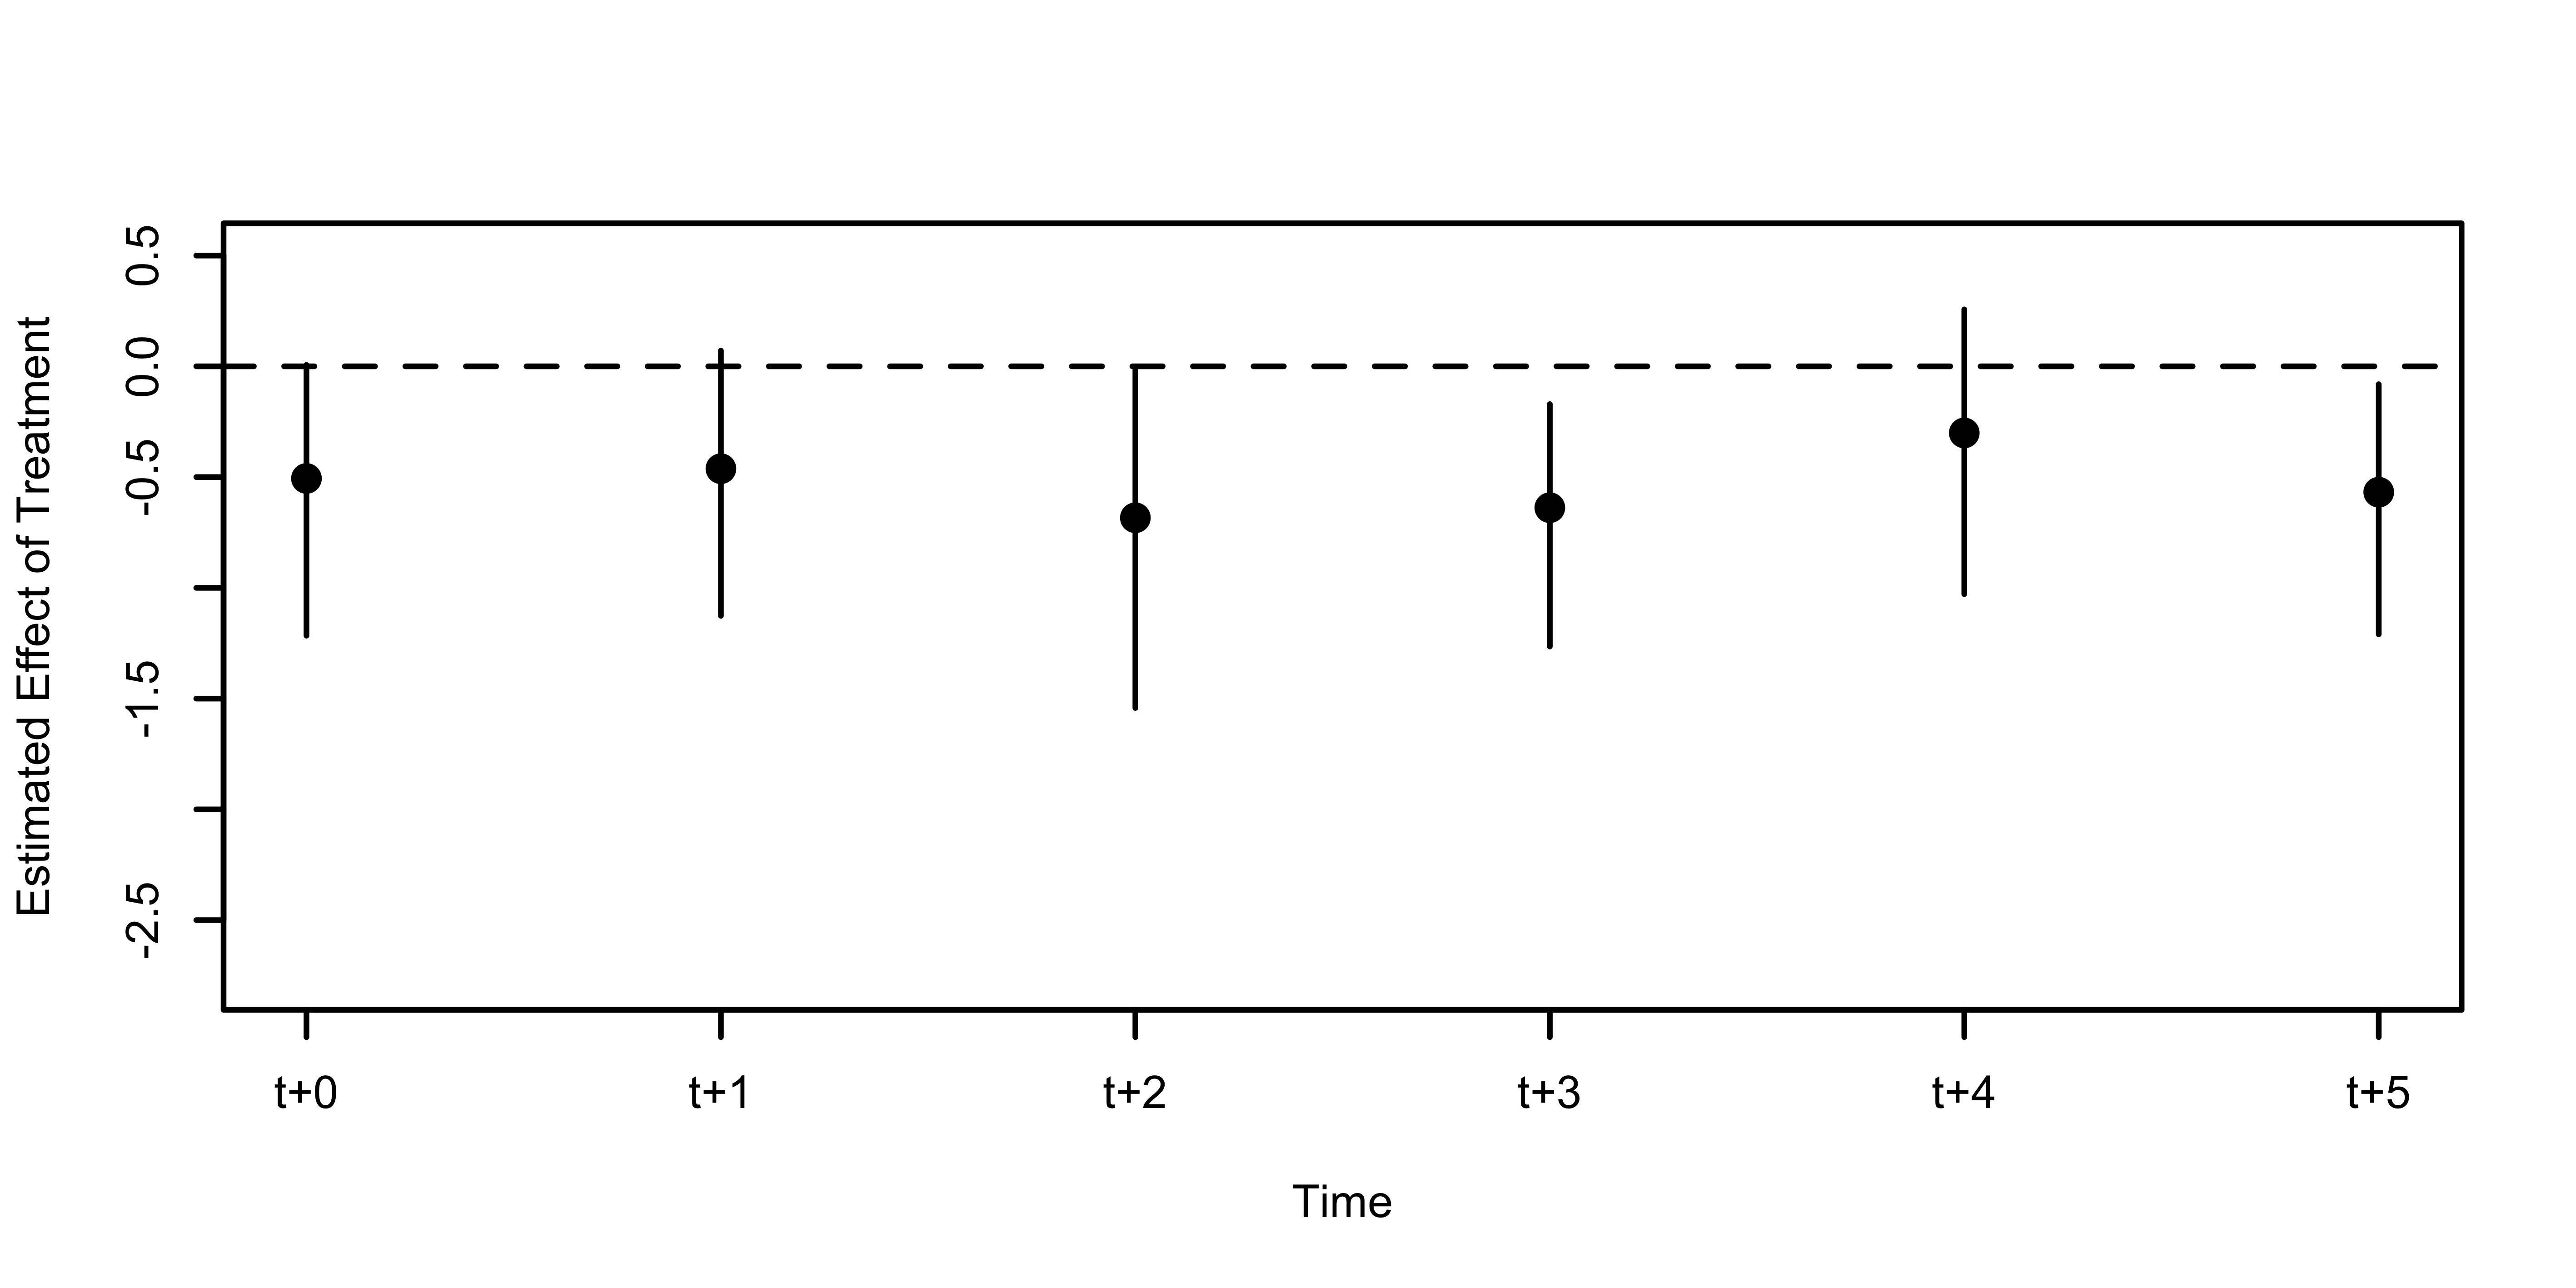
\includegraphics[width=0.8\linewidth]{\figdir/match_estimates.png}
    \label{fig:match_estimates}

    \fignote{\textwidth}{}

\end{figure}

Is estimate causal?
\begin{itemize}
    \item \citet{king2006dangers} show that there are four sources of bias
        (ommitted variable, posttreatment, interpolation, extrapolation).
    
    \item Discuss each in turn to argue that effect is causal (for our population
        of interest, which are people signing up to MDB). 
\end{itemize}


\subsection{Alternative window lengths}%
\label{sub:alternative_window_lengths}

\subsection{Subgroups}%
\label{sub:subgroups}

To analyse which groups benefit most from adopting Money Dashboard, we split
our sample by gender, generation, income quartiles, and pre-adoption savings
behaviour.

We define generations as follows: boomers were born between 1946 and 1964, Gen
X between 1965 and 1980, Millennials between 1981 and 1996, and Gen Z after
1997.\footnote{Based on age ranges provides by
    \href{https://www.beresfordresearch.com/age-range-by-generation/}{Beresford
Research}.}

Subgroup analysis: same Fig an Tab as in main analysis, but with line for each
subgroup. One figure for each of: gender, generations, income terciles,
per-adoption average savings tercile (inspired by \citet{carlin2017fintech},
see Fig 5 and Table 4).

See also section 6 in \citet{gargano2021goal}


\subsection{Alternative outcome variables}%
\label{sub:alternative_outcome_variables}

Look at netflows scaled by income


